% !TEX root = main.tex

\section{简介}
\subsection{分类}
机器学习(machine learning)通常可以分为以下几类:
\begin{itemize}
	\item 监督学习(supervised learning):有标签(label)
	\begin{itemize}
		\item 回归(regression):连续值
		\item 分类(classification):离散值
	\end{itemize}
	\item 无监督学习(unsupervised learning):无标签
	\begin{itemize}
		\item 降维
		\item 聚类(clustering)
	\end{itemize}
	\item 强化学习(reinforcement learning):延后的标签
\end{itemize}

\subsection{历史}
\begin{itemize}
	\item 推理期(1950-1970):逻辑理论家(Logic Theorist)A.~Newell \& H.~Simon(1975图灵奖)
	\item 知识期(1970s):知识工程之父E.~A.~Feigenbaum(1994图灵奖)
	\item 学习期(1980s):决策树、归纳逻辑程序设计(Prolog)
\end{itemize}

机器学习的五大学派(tribe):
\begin{itemize}
	\item 符号主义(symbolist)
	\item 联结主义(connectionist)
	\item 进化主义(evolutionaries)
	\item 贝叶斯主义(bayesians)
	\item 类比主义(analogizers)
\end{itemize}
\begin{figure}[H]
\centering
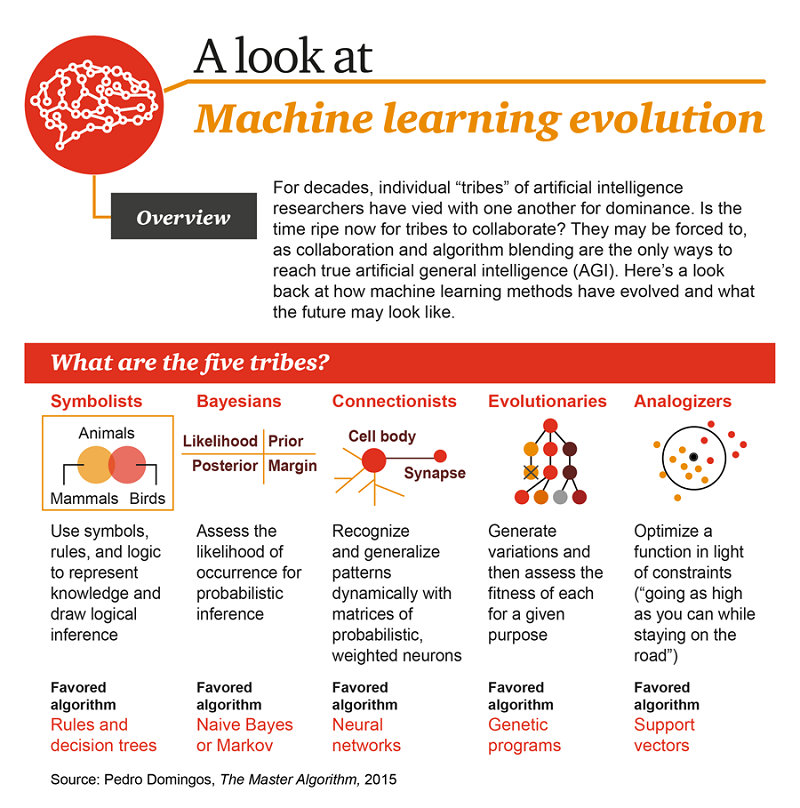
\includegraphics[width=0.8\linewidth]{fig/A-Look-at-Machine-Learning-Evolution.png}
\end{figure}